% 2019-04-01

\documentclass[10pt]{article}
\usepackage[T1]{fontenc}
\usepackage{amssymb}
\usepackage{amsmath}
\usepackage{graphicx}
% \begin{figure}[h]
% \centering
% \includegraphics[width=6.5in]{folder/photo.png}
% \caption{}
% \label{}
% \end{figure}



\usepackage{tikz}
\usetikzlibrary{arrows}
\usepackage{subfigure}
\usepackage{stackrel}
\usepackage{blindtext}

\usepackage{biblatex}
\addbibresource{library.bib}

\oddsidemargin=0.15in
\evensidemargin=0.15in
\topmargin=-.5in
\textheight=9in
\textwidth=6.25in

\usepackage[colorlinks=true,breaklinks,pdfpagemode=none,linkcolor=blue,citecolor=blue]{hyperref}

\usepackage{enumerate}
% \vspace{-6pt}
% \begin{itemize}
%     \setlength{\itemsep}{0pt}%
%     \setlength{\parskip}{0pt}%
%     \item Item 1
%     \item Item 2
%         \begin{itemize}
%             \setlength{\itemsep}{0pt}%
%             \setlength{\parskip}{0pt}%
%             \item Sublist Item 1
%             \item Sublist Item 2
%         \end{itemize}
%         \item Item 3
% \end{itemize}
% \vspace{-6pt}


\usepackage{enumitem}
\setlist{itemsep=0mm}

\usepackage{amsmath,amsfonts,amssymb,bm}

\usepackage{scrextend}

\begin{document}

   \noindent
   \begin{center}

   \hrulefill
   
   \vspace{5pt}
   
   \makebox[\textwidth]{ {\bf Energy Systems Analysis} \hfill  A.D. Smith 2019}
   \vspace{0pt}
   
   {\Large \hfill  Lecture 28. Supply and Demand: Electrical and Thermal Energy}
   \vspace{5pt}
   
  
   \hrulefill
   \end{center}
   
   
   {\color{darkgray}{\center{ \small{      ``A rapid evolution is underway
in the electricity sector that will also have a significant impact on the \\buildings sector.''
\\%[3pt]
\rightline{{\rm --- ASHRAE President Sheila Hayter in report ``Building Our New Energy Future'' \cite{newenergyfuture}}}}}}}
   



\section{Supply and Demand: Electrical Energy}




Dynamic changes in the energy sector and the power generation sector in recent years have brought the importance of matching supply and demand in terms of timing and location to the forefront. The makeup of generators is rapidly changing, the load profiles within buildings are also changing, and sensor data and data analytics are opening up new opportunities for managing this complex interconnected system of systems. Digital meters are increasingly able to acquire and process more information, and are more often being equipped with communications capabilities that allow the surrounding electrical network to receive information about how the loads fluctuate or to communicate information about how the load might be asked (or required) to respond to grid conditions \cite{newenergyfuture}.

Recall from Lecture 21 that we defined
capacity factor of electricity generation as ``a measure (expressed as a percent [or a fraction between 0 and 1]) of how often an electricity generator operates during a specific period of time using a ratio of the actual output to the maximum possible output during that time period.'' % https://www.eia.gov/tools/faqs/faq.php?id=101&t=3
The capacity factor is a critical piece of information in today's dynamic electricity sector, because \textit{capacity} (the kW, MW, or GW that your generator is capable of generating) doesn't tell us anything about \textit{how often} it will be generating power, or at \textit{what specific times} it will be generating.

That's a big deal because we prefer to have power at exactly the time we want it, and grid operators must maintain a stable system even as generators turn on and off, loads turn on and off, and equipment and weather throw additional unpredictable factors into the mix. We'll look in the next lecture in more detail at what options are out there on the `demand side,' which includes buildings. In the electricity sector, the U.S. Energy Information Administration (EIA) recently summed up the changes in this way:

\begin{quote}
    The power sector experiences a notable shift in fuels used to generate electricity, driven in part by
historically low natural gas prices. Increased natural gas-fired electricity generation; larger shares of
intermittent renewables; and additional retirements of less economic existing coal and nuclear plants
occur during the projection period. \cite{aeo2019}
\end{quote}

Figure \ref{USgen} illustrates historical and projected future changes in the makeup of electrical generation for the U.S. Note that these are capacity additions and that the solar PV generator will necessarily operate at a lower capacity factor than, for example, a natural gas baseload generator.

            \begin{figure}[h]
            \centering
            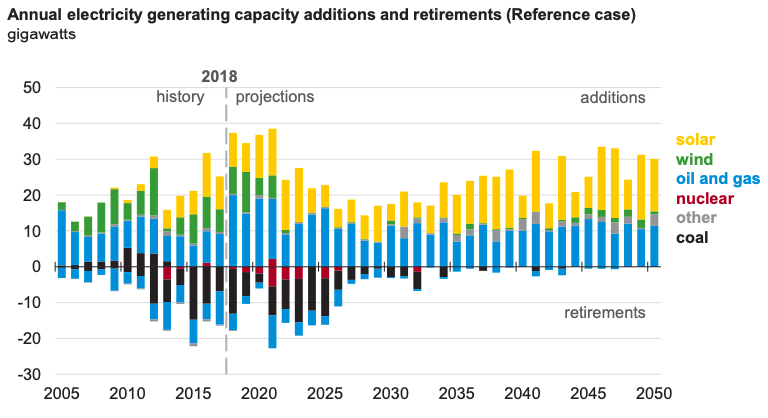
\includegraphics[width=13cm]{extras28/annelec.png}
            \caption{Expected requirements for new generating capacity in the United States \cite{aeo2019}}
            \label{USgen}
            \end{figure}

\subsection{Buildings and the Electrical Grid}

As the current ASHRAE president points out in the quote opening these lecture notes, the changes that the electricity sector faces will necessary affect the buildings that rely on grid generation to operate as designed. There is a growing awareness among many in both the buildings sector and the electricity sector that maintaining security and reliability as both sectors transition to a more modern and less carbon-intensive energy system will require cooperation and joint planning between the two ``sides.'' Because these sectors historically haven't had to interact as much, they tend to quantify things differently: 

\begin{quote}
The end-use sectors have different representative metrics for demand used to estimate energy
intensity---number of households for the residential sector, floorspace for the commercial sector, industrial
value of shipments for the industrial sector, and travel metrics for the transportation sector. 
\cite{aeo2019}
\end{quote}

Note that the transportation sector is also relevant to the management of the combined electricity sector-built environment system, particularly when we consider that electric fleets and natural gas-fueled vehicles are in more widespread use.

\subsection{Solar PV}

A \textit{grid-connected distributed solar PV system} will inject power into the grid when it produces more than the building is currently using (a ``power export'' from the perspective of the building). When PV systems are close together geographically and in terms of their location in the electrical network, these sudden influxes of power must be managed by distribution system operators to maintain stability and reliable delivery of power to their other customers. The \textit{duck chart}  is the most famous example illustrating ``the need to fully integrate distributed resources into grid system planning and operations to allow maximum use of variable generation.'' \cite{noauthor_undated-wm}. The California ISO, credited with naming this characteristic shape the ``duck curve'' \cite{noauthor_undated-wm}, faces challenges due to the accelerated growth of solar PV and other renewables when compared with the rest of the continental U.S. states, including ``short
steep ramps of increasing or decreasing demand, risk
of oversupply of electricity, and decreased frequency
response that can impact grid reliability'' \cite{newenergyfuture}. The addition of electrical energy storage (EES), a.k.a. batteries, can provide additional benefits above and beyond those of a solar PV generation system alone, by increasing the portion of the building's electric load that the PV + EES system is able to meet, or by increasing the percentage of PV-generated electricity that is consumed on site \cite{OShaughnessy2018-gu}. 

\subsection{Combined Heat and Power}
\label{chpe}

The EIA predicts that after solar PV, combined heat and power (CHP), (also known as cogeneration, explained in Lecture 22), is expected to expand faster than other forms of distributed generation between now and 2050 \cite{aeo2019}. CHP can be operated to follow the electric load to try and meet as much of the building's electrical load profile as possible. The ability to modulate the load depends on the individual technology (e.g. diesel engine or gas turbine) and the ability to meet the demand at any given instant also depends on the magnitude of the demand compared with the generator's current capacity. Typically generators are referenced using a capacity determined at standard reference conditions, such as 68$^{\circ}$F and 14.7 psi, but their ability to generate at a given time depends on their \textit{availability} (whether they are currently offline for maintenance or other reasons) and, for heat engines, on ambient conditions (air intake temperature, pressure, and moisture content). 




\section{Supply and Demand: Thermal Energy}

While a mismatch between thermal energy demand and supply may have such dramatic immediate consequences, and certainly doesn't receive as much attention as, a similar mismatch in terms of electricity; current technology also allows for energy, emissions, and cost savings by aligning supply and demand. In the buildings sector, thermal energy requirements refer to the need to deliver heat to the space or to cool the space, or to deliver heat for processes like domestic hot water.

A building has \textbf{thermal mass} that will store heat due to the heat capacity of the materials used to construct it (as well as the material properties of the masses inside of it, like furniture). The greater the building's thermal mass, the less we would expect to see temperature fluctuations indoors when we have external temperature fluctuations. Of course, the effects due to thermal mass interact with changes due to HVAC operations and infiltration or exfiltration. If the building heats up or cools down slowly, that's generally a good sign for maintaining indoor conditions like thermal comfort, but it means that it will be a slower process to ``shift'' thermal loads in time.

\subsection{Solar Thermal Energy}

We might think of solar thermal collectors for heating as being analogous to solar PV generators for electricity. Collectors are a form of \textbf{active solar}, meaning that they are mechanical systems requiring active management of a fluid that absorbs solar radiation and then is circulated to transfer that heat to a building space or to a thermal storage device \cite{noauthor_undated-zq}.

Solar thermal collectors can be divided into two major types:

\begin{labeling}{Nonconcentrating collectors xxx}
\item [\textbf{Nonconcentrating collectors}] ``The collector area (the area that intercepts the solar radiation) is the same as the absorber area (the area absorbing the radiation). Solar systems for heating water or air usually have nonconcentrating collectors. \textit{Flat-plate collectors} are the most common type of nonconcentrating collectors for water and space heating in buildings and are used when temperatures lower than 200$^{\circ}$F are sufficient.''\cite{noauthor_undated-zq}
\item [\textbf{Concentrating collectors}] ``The area intercepting the solar radiation is greater, sometimes hundreds of times greater, than the absorber area. The collector focuses, or concentrates, solar energy onto an absorber. The collector usually moves so that it maintains a high degree of concentration on the absorber.'' \cite{noauthor_undated-zq} These are more common in concentrating solar power plants, where the ultimate goal is electricity generation, rather than in distributed solar applications.

\\
\end{labeling}


The alternative to active solar is \textbf{passive solar}, which refers to building design elements that take solar gains into account in a way that benefits the thermal regulation of the indoor environment. These could include trombe walls \cite{noauthor_undated-yi}, careful placement of south facing windows, overhangs or shades \cite{noauthor_undated-zq}. Note that passive solar changes both the ``supply'' of heat (by guiding more or less solar radiation and, therefore, heat into the conditioned space) as well as the ``demand'' for heating or cooling.

\subsection{Combined Heat and Power}
\label{chph}

CHP can also be operated to follow the thermal load to try and meet as much of the building's thermal load profile as possible. The ability to modulate the generator's output depends on the same external factors as in Section \ref{chpe}, as well as the effectiveness of the heat exchangers conveying excess heat from the generator to the thermal loads it serves (e.g. space heating or water heating). The addition of thermal storage (TS) can provide additional benefits above and beyond those of a CHP generator and heat recovery system alone, by increasing the portion of the building's heating load that the CHP + TS system is able to meet \cite{Smith2013-xo}.

% license
\bigskip

\noindent
\texttt{\footnotesize RESTRICTED PUBLIC LICENSE --- READ BEFORE SHARING. This is a draft version made available by Amanda D. Smith under a Creative Commons Attribution-NonCommercial-ShareAlike license. 
\href{https://creativecommons.org/licenses/by-nc-sa/4.0/}{CC BY-NC-SA 4.0}}

% references
\newpage
\printbibliography

\end{document}